\documentclass[a4paper,12pt]{scrartcl}
\usepackage[utf8]{inputenc}
\usepackage[T1]{fontenc}
\usepackage[german]{babel}
\usepackage{listings}
\usepackage{xcolor}
\usepackage{amsmath,amsfonts,amsthm,bm,graphicx}
\usepackage{tikz,pgfplots}
\usepackage{listings}
\usepackage{stmaryrd}
\usepackage{rotating}
\usepackage{listings}
\usepackage{hyperref}
\usepackage{svg}
% Einstellungen für Quellcode
\lstset{
basicstyle=\ttfamily\footnotesize,
keywordstyle=\color{blue},
commentstyle=\color{gray},
stringstyle=\color{green!60!black},
numbers=left,
numberstyle=\tiny,
stepnumber=1,
tabsize=2,
breaklines=true,
frame=single
}

\begin{document}

\section*{Aufgabe 1: Iris-Klassifikation}

\textbf{Ziel:} Klassifikation der Iris-Blumen in die drei Arten \textit{setosa}, \textit{versicolor} und \textit{virginica}.\

\textbf{Vorgehen:} Zunächst wurde der Iris-Datensatz geladen. Anschließend erfolgte eine Aufteilung in Trainings- (80) und Testdaten (20) mit festem Seed (R: \lstinline|set.seed(42)|, Python: \lstinline|random_state=42|, RapidMiner: \lstinline|random_seed=42|).

Zur Modellbildung wurde in R der folgende Befehl verwendet:\\
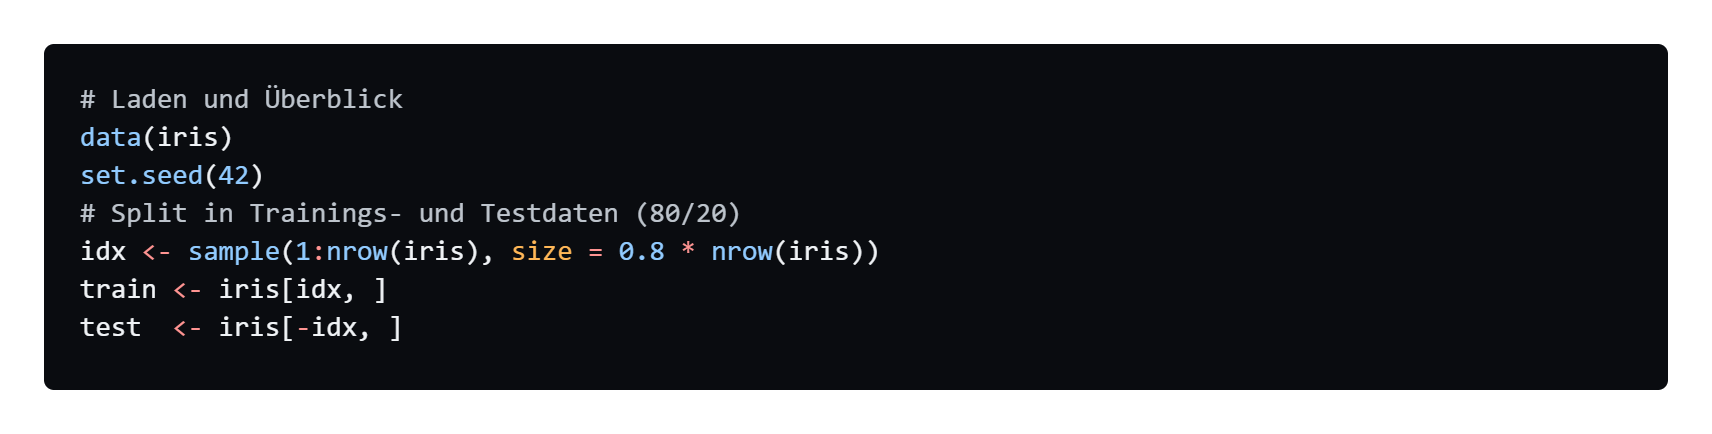
\includegraphics[scale=0.25]{iris_1_R.png}\\

In Python kam folgender Code zum Einsatz:\\
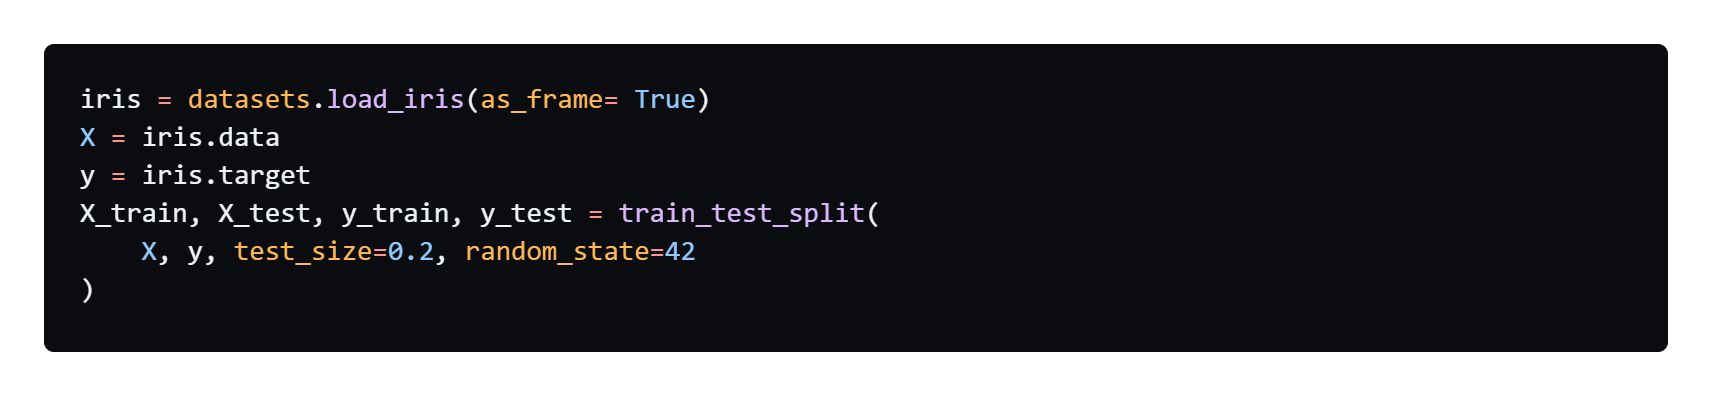
\includegraphics[scale= 0.25]{iris_1_py.png}\\
In Orange wurde der Workflow mit den Modulen File $\to$ Data Sampler (80/20) $\to$ Random Forest $\to$ Test \& Score realisiert. In RapidMiner wurde ein äquivalenter Prozess mit den Schritten Read CSV $\to$ Split Data $\to$ Random Forest $\to$ Apply Model $\to$ Performance umgesetzt.

Zur Evaluation wurden Metriken wie Accuracy, Precision, Recall, F1-Score und die Confusion Matrix herangezogen.\\
In R:\\
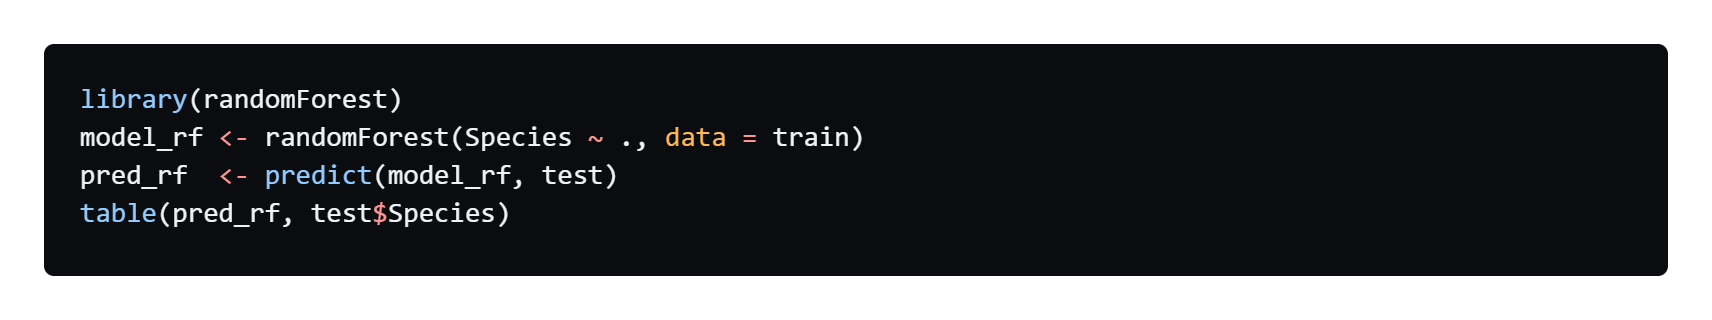
\includegraphics[scale=0.25]{iris_2_R.png}\\
In Python:\\
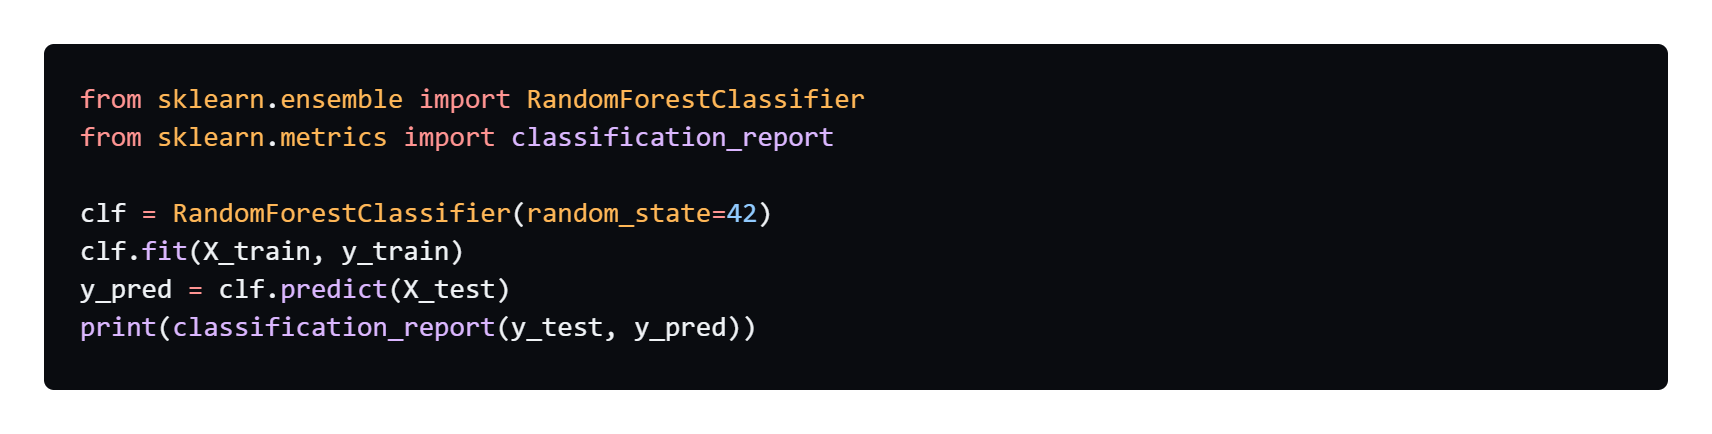
\includegraphics[scale=0.25]{iris_2_py.png}\\
\newline
\textbf{Ergebnisse (Python/R):}\\
R:
\begin{table}[!h]
\begin{tabular}{lllll}
pred\_rf   & setosa & versicolor & virginica &  \\
setosa     & 9      & 0          & 0         &  \\
versicolor & 0      & 10         & 1         &  \\
virginica  & 0      & 1          & 9         & 
\end{tabular}
\end{table}

Python:
\begin{table}[!h]
\begin{tabular}{lllll}
precision    & recall & f1-score & support &    \\
virginica    & 1.00   & 1.00     & 1.00    & 10 \\
setosa       & 1.00   & 1.00     & 1.00    & 9  \\
versicolor   & 1.00   & 1.00     & 1.00    & 11 \\
accuracy     & 1.00   & 30       &         &    \\
macro avg    & 1.00   & 1.00     & 1.00    & 30 \\
weighted avg & 1.00   & 1.00     & 1.00    & 30
\end{tabular}
\end{table}
\newline
\textbf{Interpretation:} Das Modell zeigt eine sehr gute Trennschärfe, insbesondere zwischen \textit{setosa} und den anderen beiden Arten.


\section*{Aufgabe 2: Algorithmusvergleich (Decision Tree, Naive Bayes, SVM)}

\textbf{Ziel:} Vergleich der Klassifikationsleistung dreier Algorithmen auf demselben Datensatz und Splits.\

\textbf{Vorgehen:} Als Datenbasis diente erneut der Iris-Datensatz. Die Daten wurden wie in Aufgabe 1 aufgeteilt. Es wurden drei Modelle trainiert:

\textbf{Decision Tree:} R: \lstinline|rpart()|, Python: \lstinline|DecisionTreeClassifier()|, Orange: Decision Tree-Widget, RapidMiner: Decision Tree $\to$ Apply Model.

\textbf{Naive Bayes:} R: \lstinline|e1071::naiveBayes()|, Python: \lstinline|GaussianNB()|, Orange: Naive Bayes-Widget, RapidMiner: Naive Bayes $\to$ Apply Model.

\textbf{SVM:} R: \lstinline|e1071::svm()|, Python: \lstinline|SVC()|, Orange: SVM-Widget, RapidMiner: SVM $\to$ Apply Model.

Die Modelle wurden mit Accuracy, Precision, Recall, F1 und ROC-AUC (für binäre und multiklassige Klassifikation) verglichen.\\
Hier als Beispiel der Decision Tree der durch das Python script erzeugt wurde:\\
\begin{figure}[htbp]
  \centering
  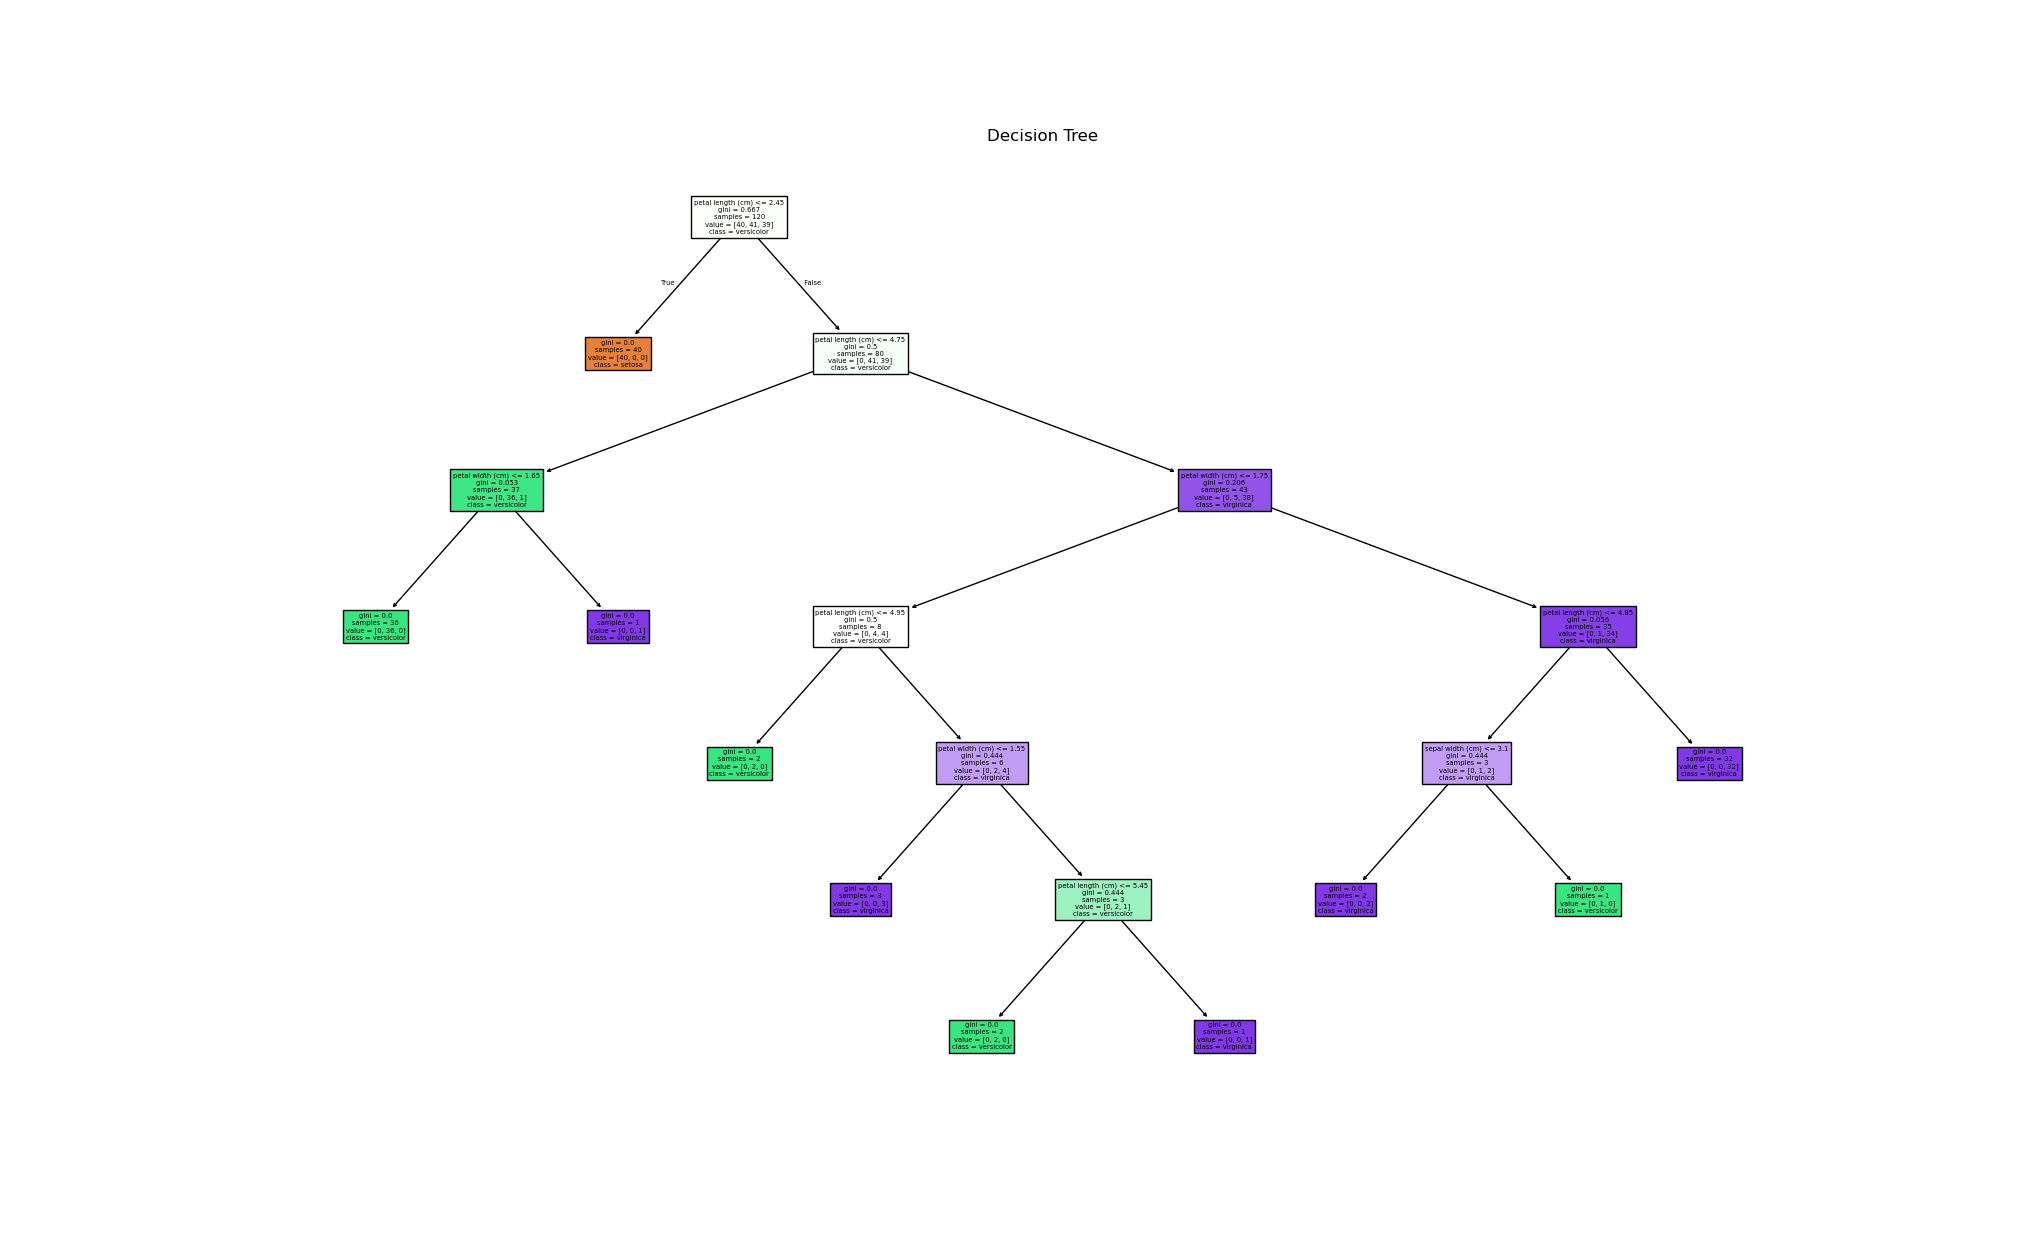
\includegraphics[scale=0.29]{Decision_tree.png}
  \caption{Auf meinem Discord ist das ganze auch noch mal in Hochauflösender}
\end{figure}



\textbf{Interpretation:} Alle Confusion Matrizen sind genau so wie die obigen aus Aufgabe 1 heißt alle classen wurden richtig zugeordnet.
\newpage

\section*{Aufgabe 3: Unüberwachtes Clustering (Rotwein-Daten)}

\textbf{Ziel:} Strukturen in den Rotwein-Daten entdecken mittels K-Means und hierarchischem Clustering.\

\textbf{Vorgehen:} Zunächst wurden fehlende Werte im Datensatz behandelt und eine Z-Score-Normalisierung auf alle Merkmale angewendet. Zur Bestimmung der optimalen Cluster-Anzahl wurde ein Elbow-Plot (Within-Cluster-Sum-of-Squares) sowie der Silhouette-Score berechnet.

Es kamen zwei Clustering-Methoden zum Einsatz:

\textbf{K-Means:} R: \lstinline|kmeans()|, Python: \lstinline|KMeans()|, Orange: K-Means-Widget, RapidMiner: K-Means-Operator.

\textbf{Hierarchisches Clustering:} Mit Ward-Linkage in allen Tools verfügbar.

Zur Auswertung wurden die Silhouette-Scores, Cluster-Profile (Mittelwerte je Cluster) sowie Visualisierungen wie Dendrogramme und PCA-Plots genutzt.

\textbf{Ergebnisse (Beispiel):} Die optimale Clusterzahl war k = 3. Die Cluster unterschieden sich insbesondere im Phenol-Gehalt.

\textbf{Interpretation:} Es zeigten sich zwei Cluster mit hohem bzw. niedrigem Phenolgehalt und ein intermediäres Cluster.

\newpage

\section*{Aufgabe 4: Google Trends Clustering}

\textbf{Ziel:} Regionale Suchmuster in Google Trends-Zeitreihen clustern.\

\textbf{Vorgehen:} Zunächst wurde ein CSV-Export aus Google Trends geladen. Fehlende Werte wurden entfernt oder imputiert. Anschließend wurden die Daten normalisiert.

Die Feature-Matrix bestand aus Regionen als Beobachtungen und Zeitpunkten bzw. Suchbegriffen als Merkmalen. Für das Clustering wurden erneut K-Means und hierarchisches Clustering (siehe Aufgabe 3) genutzt. Zur Visualisierung wurden PCA-Scatterplots und Kartenplots eingesetzt (z.,B. mit Python \lstinline|geopandas| oder dem Geo-Widget in Orange).

\textbf{Ergebnisse (Beispiel):} Drei Cluster konnten identifiziert werden: Regionen mit saisonalen Peaks, mit stabilen Suchvolumina sowie mit volatilen Trends.

\textbf{Interpretation:} Die Cluster spiegeln typische geografische Nutzungsmuster wider, z.,B. Urlaubsregionen mit Saisonalität im Vergleich zu dauerhaft populären oder wenig frequentierten Regionen.

\vspace{1em}
\noindent\textit{Hinweis: Alle Arbeitsschritte wurden in R, Python (scikit-learn), Orange und RapidMiner (Repdiminer) implementiert, um Tool-typische Unterschiede in Usability und Konfigurationsmöglichkeiten zu vergleichen.}

\end{document}
